\chapter{ベクトル空間と線型写像}

\lectureinfo{2015年6月10日 1限}
\vspace{-0.8zw}

\section{はじめに}

「数理科学基礎」の授業が終わり、いよいよ線型代数学\footnote{すごく今更ですが、「線\uline{型}代数」と「線\uline{形}代数」は同じ意味で、どっちの漢字を使うかは気分の問題でしかありません。授業名は「線\uline{形}代数学」になってますが、このプリントでは「線\uline{型}代数」を使います。}の授業が始まりました。既に行列の計算法を学び、線型空間や線型写像出てはきましたが、この先は一段と重たい計算や抽象的な議論が出てきます。心してかかってください。

抽象的な議論をする理由は、ひとえに「適用範囲が広がるから」です。普通に行列を計算しているだけでもそれなりに得られるものはあるのですが、線型空間と線型写像の言葉によって、行列計算のテクニックを他の様々な場面に応用することができます。そしてこれから見ていくように「線型な場面」というのは多々あるので、線型代数を理解しているとこの先の人生で非常に役立ちます。

一方で「\textbf{線型空間と線型写像は、それぞれ数ベクトル空間と行列がモデルになっている}」という事実を忘れてはいけません。抽象論ばかりやっていると時々自分が何をしているのか分からなくなってきますが、そういう時は必ず「行列だったらどうだろう」と考えてみましょう。特に、最も手頃な$2$次正方行列で試してみると良いと思います。

\paragraph{今回の内容について}

今回配付するプリントの分量は、いつもの$2$倍くらいの厚さになってしまいました。おそらく\textbf{今回は、$1$年間の授業全体を通して一番難易度の勾配が急}なところだと思います。最終的には全て理解することが望ましいですが、一度に理解するのは厳しいかもしれません。そういうときは、次のようにしてみてください。
\begin{itemize}
\item 線型空間と線型写像の定義は、$\mathbb{R}^2$の部分空間や$1$次函数の例などを使い、確実に理解してください。これが分かっていないとにっちもさっちもいきません。
\item 部分空間の定義も、分からないと後々困ります。また最低限、連立一次方程式の解空間が部分空間になっていることは理解してください。
\item 多項式の空間、数列の空間と函数空間は「数ベクトル空間ではない線型空間の例」として典型的なものです。そういう意味でこれらの問題は重要なのですが、数ベクトル空間のことをよく理解していないと、勉強するのは大変だと思います。今取り組むのが大変だと思ったら、後で戻ってきてください。
\item 多項式の空間は、数列の空間と函数空間に比べて扱いやすいと思います。また数列の空間と函数空間のどちらが分かりやすいかについては、人によって個人差がありそうです。好きな方から取り組みましょう。
\end{itemize}

また毎週のレポート問題に取り組むにあたっては、\textbf{自分が理解できる問題を着実に解くこと}が大事です。特にこれから先、色々な命題を\textbf{定義に基づいてきっちり示す}ことが問われます。ですから生半可な気持ちで雑に解いたり、まして他人の答案を (間違ったまま) 書き写したりすることは全く無意味です\footnote{誰とは言いませんが、たとえばベクトル空間のことを「ベクトル場」と言い間違えている答案が$5$枚以上ありました。こういうミスがあると、採点してる側には「何も考えずに誰かのを書き写している」ということが一発で見えてしまいます。}。それよりは「何が分からなかったか」をはっきりさせる方が大事でしょう。こういう点を意識して、きちんとレポートに取り組んでください。

\section{線型空間と線型写像}

これからの主役は言うまでもなく線型空間と線型写像です。まずそれらの定義を確認し、それから「線型空間の中に入っている、より小さな線型空間」に関する考察をしましょう。

\subsection{線型空間の定義と例}

\paragraph{線型空間の定義 (再掲)} \label{def:vector_space}

次の条件を満たす集合$V$を\textbf{線型空間}あるいは\textbf{ベクトル空間}というのでした。

\begin{itemize}
\item $V$上に加法が定義されており
\begin{itemize}
\item 任意の$\bm{u}, \bm{v}, \bm{w}\in V$に対し$(\bm{u} + \bm{v}) + \bm{w} = \bm{u} + (\bm{v} + \bm{w})$が成り立つ\footnote{このように「演算の結果が順番に依存しない」ということを指して、\textbf{結合法則}が成り立つといいます。}
\item 任意の$\bm{u}\in V$に対し$\bm{u} + \bm{0} = \bm{0} + \bm{u} = \bm{0}$となる$\bm{0}\in V$が唯一存在する
\item 任意の$\bm{u}\in V$に対し、$\bm{u} + \bm{v} = \bm{0}$となる$\bm{v}\in V$が唯一存在する (この$\bm{v}$を$-\bm{u}$と書く)
\item 任意の$\bm{u}, \bm{v}\in V$に対し$\bm{u} + \bm{v} = \bm{v} + \bm{u}$が成り立つ
\end{itemize}
\item $V$上にスカラー倍が定義されており
\begin{itemize}
\item 任意の$\alpha, \beta\in\mathbb{R}$と$\bm{v}\in V$に対し$\alpha(\beta\bm{v})=(\alpha\beta)\bm{v}$が成り立つ
\item 任意の$\bm{v}\in V$に対し、$1\bm{v}=\bm{v}$が成り立つ
\end{itemize}
\item スカラー倍と和が分配法則を満たす: 
\begin{itemize}
\item 任意の$\bm{u}, \bm{v}\in V$と$\alpha\in\mathbb{R}$に対し$(\alpha + \beta)\bm{v} = \alpha\bm{v} + \beta\bm{v}$
\item 任意の$\bm{u}\in V$と$\alpha,\beta\in\mathbb{R}$に対し、$\alpha(\bm{u} + \bm{v}) = \alpha\bm{u} + \alpha\bm{v}$
\end{itemize}
\end{itemize}

これらの性質から、$0\bm{v}=\bm{0}$, $(-1)\bm{v} = -\bm{v}$が成り立つことに注意しておきます:
\begin{itemize}
\item $0 \bm{v} = (0 + 0) \bm{v} = 0\bm{v} + 0\bm{v}$の両辺に$-(0\bm{v})$を足して、$\bm{0} = 0\bm{v} + \bm{0} = 0\bm{v}$を得る。
\item $\bm{0} = 0\bm{v} = \bigl(1 + (-1)\bigr)\bm{v} = \bm{v} + (-1) \bm{v}$より、$-\bm{v} = (-1)\bm{v}$を得る。
\end{itemize}

\paragraph{$\mathbb{R}^2$の部分空間の例} ここで、線型空間の何たるかを目で見て理解するため「平面$\mathbb{R}^2$の部分集合で、線型空間になっているものは何か」を考えてみましょう。次に挙げる$3$つの部分集合のうち、どれが線型空間でしょうか?\footnote{すぐ後ろで議論はしますが、それを読む前に自分で定義に従って、どれが線型空間か判定してみると良いと思います。}
\begin{align*}
V_1 := \biggl\{ \begin{pmatrix} x \\ y \end{pmatrix} \in \mathbb{R}^2 \mid y = 2x \biggr\}, \qquad
V_2 := \biggl\{ \begin{pmatrix} x \\ y \end{pmatrix} \in \mathbb{R}^2 \mid y = x - 1 \biggr\}, \qquad
V_3 := \biggl\{ \begin{pmatrix} x \\ y \end{pmatrix} \in \mathbb{R}^2 \mid y = x^2 \biggr\}
\end{align*}
\begin{figure}[h!tbp]
\centering
\begin{picture}(0,0)
\put(40.8, 74){\circle*{2}}
\put(40.8, 74){\vector(1,2){25}}
\end{picture}
\subfigure[$y = 2x$]{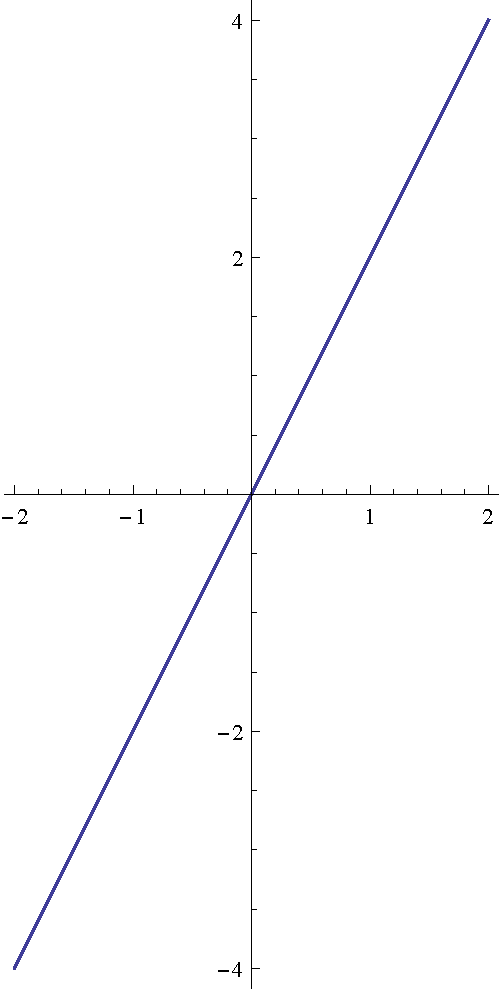
\includegraphics[height = .3\textwidth]{20150610-fig1-1.pdf}}\ 
\begin{picture}(0,0)
\put(76.6, 76.7){\circle*{2}}
\put(76.6, 76.7){\vector(1, 0){35.8}}
\put(76.6, 76.7){\vector(0, -1){36.5}}
\put(76.2, 76.5){\vector(1, -1){36.1}}
\put(76.6, 40.1){\dashbox(35.5, 36.6){}}
\end{picture}
\subfigure[$y = x - 1$]{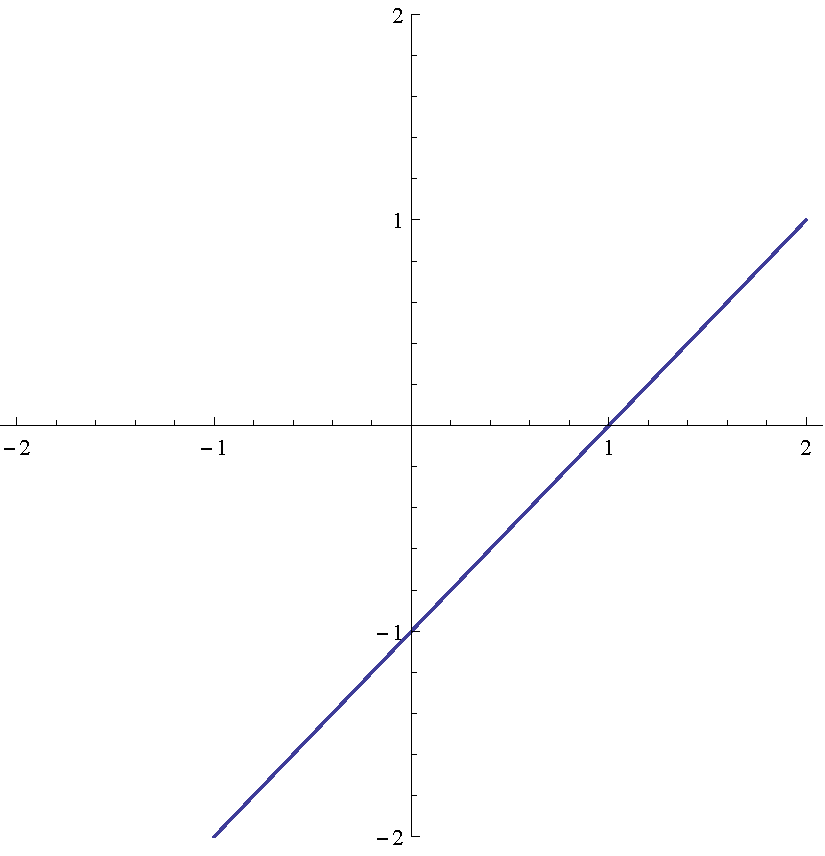
\includegraphics[width = .3\textwidth]{20150610-fig1-2.pdf}}\ 
\begin{picture}(0,0)
\put(77.5, 39){\circle*{2}}
\put(77.5, 39){\vector(1, 1){36}}
\put(77.5, 39){\vector(1, 1){72}}
\end{picture}
\subfigure[$y = x^2$]{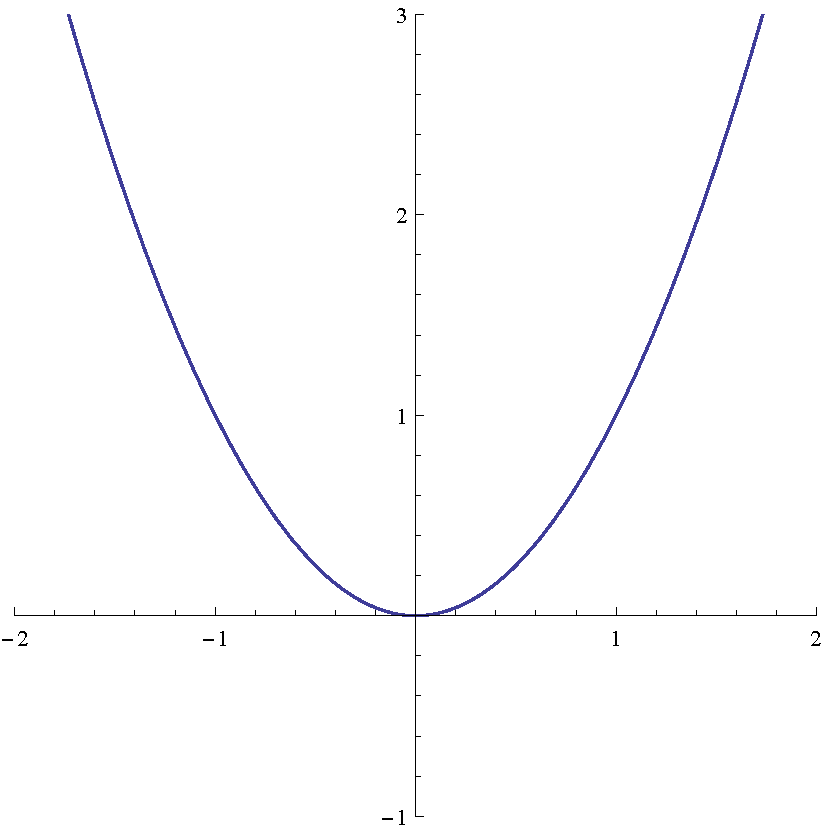
\includegraphics[width = .3\textwidth]{20150610-fig1-3.pdf}}
\end{figure}

%あとで picture 環境で矢印を重ねる

まず$V_3$の放物線$y = x^2$は、見るからに線型じゃなさそうな格好をしています。実際、$\bm{v} := {}^t (1,1)$は放物線の上に乗りますが、$2$倍した$2\bm{v} = {}^t (2,2)$は放物線からはみ出します。よってこれは線型空間の定義を満たしません。

次に$V_1$の直線$y = 2x$は、いかにも線型と呼ぶにふさわしい図形です。そして実際、ちゃんと線型空間になります。この直線上の点は${}^t (x, 2x)$という格好で書けます。そこで直線上のベクトル${}^t (a, 2a)$と${}^t (b, 2b)$を取ってくると、これらの和${}^t \bigl(a+b, 2(a+b)\bigr)$も再び直線$y = 2x$に乗ります。またスカラー倍も$\alpha {}^t (a, 2a) = (a\alpha, 2a\alpha)$となり、ちゃんと直線$y = 2x$上に乗ります。絵で描いてみると、どう見ても加法とスカラー倍で閉じていることが一段と良く分かりますね。確かに$y = 2x$は線型空間でした。

ところが線型空間になるためには、単に\textbf{まっすぐならば良いというわけでもない}のです。実は直線$y = x - 1$は線型空間になっていません。たとえばベクトル${}^t (1, 0)$, ${}^t (0, -1)$はこの直線上に乗りますが、これらを足した${}^t (1, -1)$は直線$y = x -1$からはみ出してしまいます。こうして$y = x -1$は線型空間でないことが分かりました。

以上をまとめると、線型空間は\textbf{原点を持つ、まっすぐな空間}ということになります。

ちなみに線型空間の定義は、大雑把には「ベクトルの足し算できること」「ベクトルのスカラー倍ができること」に分かれます。きちんと線型空間を定義するには、このどちらの条件も必要です。たとえば成分が全て整数であるベクトルの集合$\mathbb{Z}^2 := \bigl\{{}^t(m, n)\in\mathbb{R}^2 \mid m, n\in\mathbb{Z}\bigr\}$は、加法で閉じますがスカラー倍で閉じません。また$x, y$軸と第$1, 3$象限を合わせた$\bigl\{{}^t(x, y)\in\mathbb{R}^2 \mid xy \geq 0 \bigr\}$という集合は、スカラー倍で閉じますが加法では閉じません。

\begin{figure}[h!tbp]
\centering
\subfigure[$\mathbb{Z}^2$]{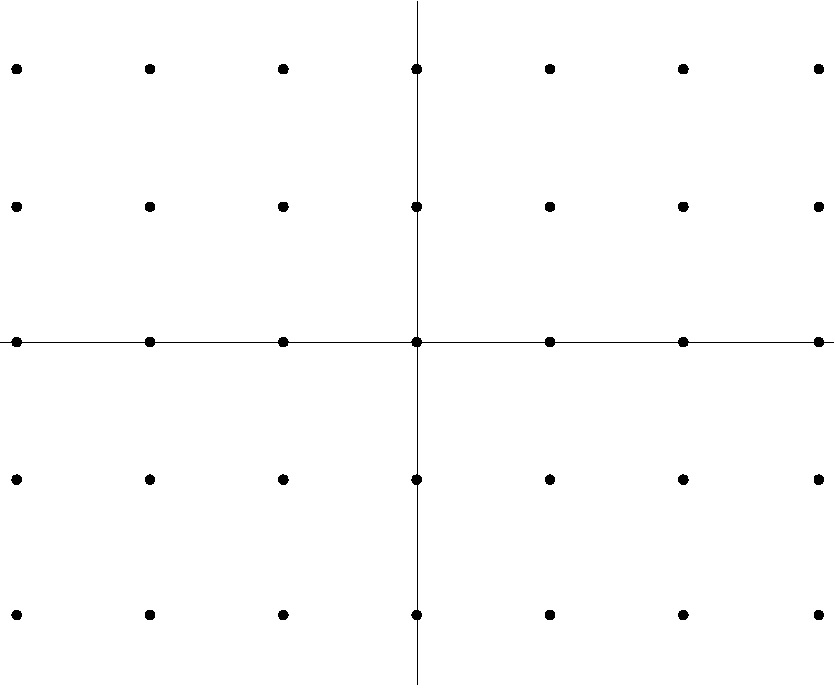
\includegraphics[width = .35\textwidth]{20150610-fig2-1.pdf}}
\begin{picture}(0,0)
\put(-89.4, 71.2){\circle*{2}}
\put(-89.6, 71.4){\vector(1, 1){28}}
\put(-89.6, 71.3){\vector(1, -2){28}}
\put(-62.1, 15.3){\vector(1, 1){28}}
\put(-62.0, 99.2){\vector(1, -2){28}}
\end{picture}
\quad
\subfigure[$xy \geq 0 $]{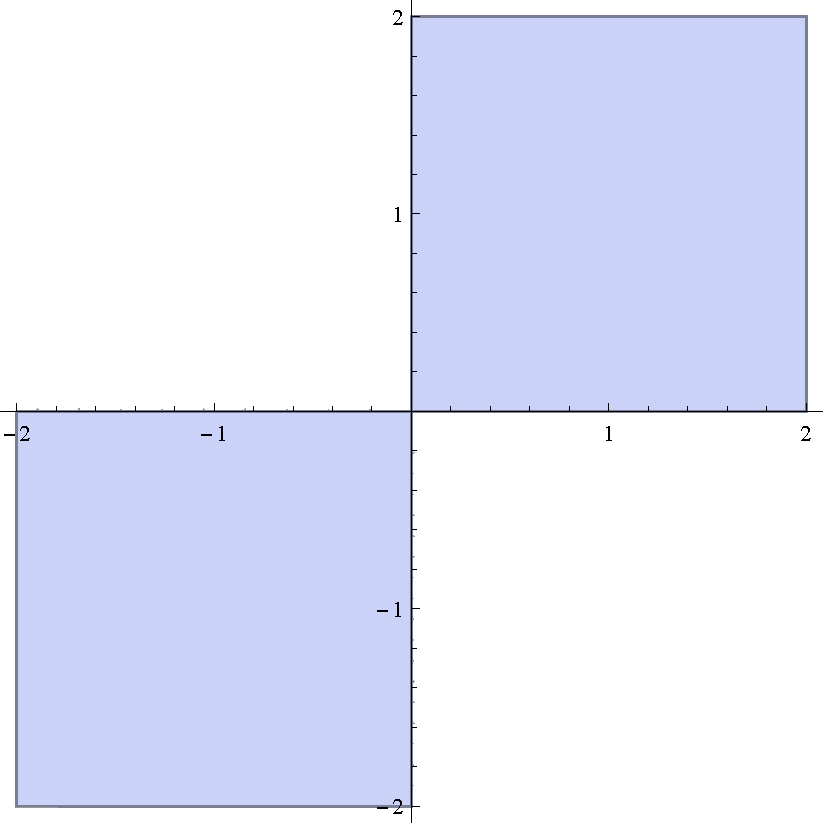
\includegraphics[width = .35\textwidth]{20150610-fig2-2.pdf}}
\end{figure}

\subsection{線型写像} \label{subsection:linear_map}

\paragraph{線型写像の定義}

$V, W$を共に線型空間とするとき、$f\colon V\rightarrow W$が線型写像であるとは
\begin{itemize}
\item 任意の$\bm{u}$, $\bm{v}\in V$に対し、$f(\bm{u} + \bm{v}) = f(\bm{u}) + f(\bm{v})$
\item 任意の$\bm{u}\in V$, $\alpha\in\mathbb{R}$に対し、$f(\alpha\bm{u}) = \alpha f(\bm{u})$
\end{itemize}
が成り立つことでした。

この定義が、何となく「線型空間と相性が良い」ことを感じて欲しいのですが、どうでしょうか?$V$と$W$は線型空間だから、どちらに対しても足し算とスカラー倍が定義されています。そして$f$が線型写像であることの条件は、\textbf{$f$を施してから足し算 / スカラー倍をしても、足し算 / スカラー倍をしてから$f$を施しても、結果が同じになる}ということを言っています\footnote{このことを称して「$f$は加法 / スカラー倍と整合的 (compatible) である」と言ったりもします。線型空間の構造と整合的な写像が線型写像、というわけです。}。図式にすると次のようになります。これを見て、線型写像と線型空間の相性の良さを感じ取ってください。
\[
\begin{tikzcd}
(\bm{v},\bm{w}) \arrow[mapsto]{r}{f\times f}  \arrow[mapsto]{d}{+} & \bigl(f(\bm{v}),f(\bm{w})\bigr) \arrow[mapsto]{d}{+} \\
\bm{v}+\bm{w} \arrow[mapsto]{r}{f} & f(\bm{v}+\bm{w})=f(\bm{v})+f(\bm{w})
\end{tikzcd}
\qquad
\begin{tikzcd}
(\alpha,\bm{v}) \arrow[mapsto]{r}{f\times f}  \arrow[mapsto]{d}{\cdot} & \bigl(\alpha,f(\bm{w})\bigr) \arrow[mapsto]{d}{\cdot}\\
\alpha\bm{v} \arrow[mapsto]{r}{f}  & f(\alpha\bm{v})=\alpha f(\bm{v})
\end{tikzcd}
\]

また$f$が線型写像なら, $f(\bm{0})=f(\bm{0}-\bm{0})=f(\bm{0})-f(\bm{0})=\bm{0}$が成り立つ\footnote{雑な書き方をしましたが, $f$の中に入る$\bm{0}$は$V$の元で, $f(\bm{0})=\bm{0}$の右辺は$W$の元です. 厳密に言えば$\bm{0}_V$, $\bm{0}_W$などと書いて区別するべきですが, 文脈から意味がはっきり取れる場合は略記して差し支えありません. }ことにも注意しておきましょう.  \textbf{線型写像は原点を原点にうつします。}

さて、前回のプリントで「行列の掛け算は線型写像である」ということを説明しました。その中で最も単純な場合、つまり$f$が$\mathbb{R}$から$\mathbb{R}$への線型写像である場合を考えましょう。前回のプリントでも少しだけ触れましたが、この場合$f$は定数項が$0$であるような$1$次函数です。裏返して言えば、正比例の関係式をベクトルに一般化したものが線型写像となります。このことをチェックしましょう。

\paragraph{問1の解答}
$f(x) := ax + b$で定まる写像$f\colon\mathbb{R}\rightarrow\mathbb{R}$が線型写像であるとする。このとき$f(x + y) = f(x) + f(y)$が成り立つので、$0 = f(x + y) - f(x) - f(y) = \{a(x + y) + b\} - (ax + b) - (ay - b) = b$となる。よって$b = 0$でないといけない。

逆に$b = 0$のとき、$f(x) = ax$は線型である。実際、任意の$x, y\in\mathbb{R}$と$\alpha\in\mathbb{R}$に対し$f(x + y) = a(x + y) = ax + ay = f(x) + f(y)$, $f(\alpha x) = a (\alpha x) = \alpha (ax) = \alpha f(x)$となっている。よって$f$が線型であることと$b = 0$とが同値になる。 \qed

\subsection{部分空間}

一般に、線型空間はその中にもっと小さい線型空間を含んでいます。一番分かりやすい例は、平面$\mathbb{R}^2$の中に含まれる$x$軸や$y$軸です。これらは共に、まっすぐで原点を通っていますね。また先ほど確認したように、$\mathbb{R}^2$の原点を通る直線はいずれも線型空間です。そこで一般に、線型空間$V$の部分集合$W\subset V$でそれ自身が線型空間になっているものを、$V$の\textbf{部分空間}といいます\footnote{$部分線型空間$とか$線型部分空間$とか呼んだりもします。どれでも意味は一緒です。}。

座標軸があるおかげで、僕たちは平面上で「$x$方向」とか「$y$方向」とかを考えることができます。それと同じように部分空間を使うと、親玉の線型空間を「こっちの空間の方向とあっちの空間の方向」というように、色々な方向に分けることができます。これから先、連立方程式や微分方程式の解空間を線型代数の手法で解析していくわけですが、その時に上手い部分空間を考えると問題を切り分けることができます。部分空間はそういう風に役に立つのです。

さて部分空間は色々なところに登場しますが、部分空間が本当に線型空間になっていることを一々定義に戻ってチェックするのは、無駄があります。実は$W$が線型空間$V$の部分空間であることは
\begin{itemize}
\item 任意の$\bm{u}, \bm{v}\in W$に対し、$\bm{u} + \bm{v} \in W$が成り立つ
\item 任意の$\bm{u}\in W$と$\alpha \in \mathbb{R}$に対し、$\alpha \bm{u}\in W$が成り立つ
\end{itemize}
という$2$条件\footnote{ちなみに$1$つ目の条件を「$W$が\textbf{加法で閉じている}」といい、$2$つ目の条件を「$W$が\textbf{スカラー倍で閉じている}」と言います。「閉じている$=$はみ出さない」という感じです。}のチェックだけで事足りるのです。そのことを、問3で確かめましょう。そうすれば今後は、部分空間の確認で楽をすることができます。

\paragraph{問3を解く前に} 問題の解答に入る前に「そもそも、この問3は何がしたいのか?」を確認しておきましょう。線型空間の公理は\pageref{def:vector_space}ページに書いた通りです。一方、問題では線型空間の部分集合が「加法とスカラー倍とで閉じること」だけを部分空間の定義としています。そして表面的には「部分空間の定義」の方が「線型空間の定義」より条件が少ないように見えますが、実はこれで十分なのだということが、問題になっているのです。ここをまず押さえてください。

そして、問題の意味を理解した上で「どうせ線型空間の部分集合なんだから条件は当然成り立つでしょ」と思った人がかなり多くいました。確かに「$3$つのベクトル$\bm{u}, \bm{v}, \bm{w}$に対して$(\bm{u} + \bm{v}) + \bm{w} = \bm{u} + (\bm{v} + \bm{w})$が成り立つこと」などは、線型空間の部分集合であるから当たり前のように成り立ちます。そういう感じで大体のことは済むのですが「$\bm{0}$ベクトルが部分空間に入ること」「逆向きのベクトルが部分空間に入ること」だけは自明ではありません。ここにどう部分空間の条件を使うかがポイントです。

細かいところですが、これらに注意して解答を読んでください。

\paragraph{問3の解答} $V$を線型空間とし、その空でない部分集合$W\subset V$が$V$の加法とスカラー倍で閉じているとする。このとき$W$が線型空間の条件を満たすことを、定義に従ってチェックする\footnote{ぶっちゃけた話、このチェックはかなりかったるいのですが、人生で一度はこのチェックをやっておかないといけません。最初のうちは大変だと思いますが、時間をかけてコツコツやってみてください。大体の場合はルーチンワークなので、何回かやれば慣れてきて、テキパキできるようになります。}。
\begin{itemize}
\item 加法について: 加法そのものは、$V$で定義されている。そして
\begin{itemize}
\item 任意の$\bm{u}, \bm{v}, \bm{w}\in W$に対し$(\bm{u} + \bm{v}) + \bm{w} = \bm{u} + (\bm{v} + \bm{w})$が成り立つことは、$V$が線型空間であることから保証される。
\item $W$は空集合ではないので、何か$1$つ元$\bm{v}\in W$が取れる。すると$W$がスカラー倍で閉じていることから、$\bm{0} = 0 \bm{v} \in W$となる。
\item $W$がスカラー倍で閉じているので、$\bm{v} \in W$のとき$-\bm{v} = (-1)\bm{v} \in W$となる。また$\bm{v} + \bm{u} = \bm{0}$となる$\bm{u}$がただ一つ存在することは、$V$が線型空間であることから保証される。
\item 任意の$\bm{u}, \bm{v}\in W$に対し$\bm{u} + \bm{v} = \bm{v} + \bm{u}$が成り立つことは、$V$が線型空間であることから従う。
\end{itemize}
\item スカラー倍について: スカラー倍そのものは、$V$の中で定義されている。そして
\begin{itemize}
\item 任意の$\bm{v} \in W$と$\alpha, \beta \in \mathbb{R}$について、$\alpha(\beta \bm{v}) = (\alpha\beta)\bm{v}$が成り立つことは、$V$が線型空間であることから保証される。
\item 任意の$\bm{v} \in W$について$1\bm{v} = \bm{v}$が成り立つことは、$V$が線型空間であることから従う。
\end{itemize}
\item 分配法則が成り立つことは、$V$が線型空間であることから保証される。
\end{itemize}
\qed

\section{重要な例}

線型空間と部分空間の定義が終わったので、具体的な例を確かめてみましょう。

\subsection{連立一次方程式の解空間}

連立$1$次方程式
\begin{align*}
a_{11} x_1 + a_{12} x_2 + a_{13} x_3 &= b_1 \\
a_{21} x_1 + a_{22} x_2 + a_{23} x_3 &= b_2
\end{align*}
は、
\[
A :=
\begin{pmatrix}
a_{11} & a_{12} & a_{13} \\
a_{21} & a_{22} & a_{23}
\end{pmatrix}, \quad
\bm{x} :=
\begin{pmatrix}
x_1 \\
x_2 \\
x_3
\end{pmatrix}, \quad
\bm{b} := 
\begin{pmatrix}
b_1 \\
b_2
\end{pmatrix}
\]
とおくと、単に$A\bm{x} = \bm{b}$と書けます。特に$\bm{b} = \bm{0}$のとき、この連立方程式は\textbf{同次系}であるといい、その解全体の集合を\textbf{解空間}といいます。

この解全体の集合を「解\uline{空間}」と呼ぶことは、次のように考えれば納得がいくのではないでしょうか。一般に空間$\mathbb{R}^3$内で、$1$次方程式は平面を定めるのでした。そして方程式を連立することは、図形の側で見れば「交わりを見ること」に相当しました。ですから$3$変数の$1$次方程式は大体の場合、$1$本で平面を、$2$本で直線を、そして$3$本で点を定めます\footnote{たまに「$3$枚の平面がの交わりが$1$直線になる」という場合が起きることがあります。これは裏返せば、連立している$3$本方程式に無駄があるという事実になります。次回以降きちんと定義しますが「連立している方程式にどれだけ無駄があるか」を測る量を行列の\textbf{階数} ($\rank$) といいます。方程式に無駄があるとその分解空間の次元が上がりますから、$\rank$の増減と解空間の次元の増減がぴったり対応します。}。数学では直線とか平面とかも一緒くたに「空間」と呼んでしまう習わしがあるので、解集合のことを解空間と呼びます。また$1$次方程式の定数項が$0$でないと、それの定める平面は原点を通りません。線型空間は\uline{原点を持つ}まっすぐな図形でしたから、連立方程式の定める図形が線型空間になるためには、定数項が全て$0$でなければいけません\footnote{「別に原点を通らなくたって、線型空間と大体同じじゃないか。それだけでのけ者にするのは可哀想だ」という意見は、全くその通りです。連立$1$次方程式$A\bm{x} = \bm{b}$の解空間は、$A\bm{x} = \bm{0}$の解空間を平行移動したものに過ぎません。こういう空間を\textbf{アフィン空間}と呼んだりします。}。

事情は$n$次元でも同じです。成分が実数の$(m,n)$型行列全体の集合を$\Mat_{m, n}(\mathbb{R})$で表します。$A\in\Mat_{m, n}(\mathbb{R})$として方程式$A\bm{x} = \bm{b}$を立てると、各成分毎に$(n-1)$次元の超平面\footnote{$1$次方程式は平面$\mathbb{R}^2$内では$1$次元の直線を、空間$\mathbb{R}^3$内では$2$次元の平面を定めます。こんな感じに$1$次方程式は$n$次元空間$\mathbb{R}^n$の中で$(n-1)$次元の図形を定めます。このとき「全体の空間に対して次元がどれくらい足りないか」を\textbf{余次元}といいます。そして$n$次元空間$\mathbb{R}^n$の中で余次元が$1$のまっすぐな空間を、\textbf{超平面}といいます。}が定まります。そして連立する方程式が増えていくたびに超平面との交わりが取られ、解空間の次元がどんどん減っていくという仕組みになっています。

この解空間がちゃんと線型空間になっていることは、図形的な考察からすればほぼ明らかですが、もう一度定義通りに確かめてみましょう。

\paragraph{問4の解答}

$A \in \Mat_{m,n}(\mathbb{R})$とし、$V:=\{\bm{x}\in\mathbb{R}^n \mid A\bm{x} = \bm{0} \}$とおく。このとき$\bm{0}\in V$より$V$は空でない。そして
\begin{itemize}
\item[(1)] $\bm{u}, \bm{v}\in V$を任意に取る。このとき$A\bm{u} = A\bm{v} = \bm{0}$なので、$A(\bm{u} + \bm{v}) = A\bm{u} + A\bm{v} = \bm{0} + \bm{0} = \bm{0}$である。よって$\bm{u} + \bm{v} \in V$となる。
\item[(2)] $\alpha\in\mathbb{R}$, $\bm{u}\in V$を任意に取る。このとき$A (\alpha\bm{v}) = \alpha (A\bm{v}) = \bm{0}$なので、$\alpha\bm{u}\in V$である。
\end{itemize}

これで$V$が$\mathbb{R}^n$の部分空間であることがチェックできた。\qed

\subsection{多項式の空間}

次に、僕たちが普段言う「空間」ではないような線型空間の典型的な例として、多項式の集合を考えてみましょう。$\mathbb{R}[x]$で、$x$を変数とする実係数$1$変数多項式全体の集合を表します。これは線型空間になります。実際
\begin{itemize}
\item 多項式には加法が定義されていて
\begin{itemize}
\item 任意の多項式$f(x), g(x), h(x)\in\mathbb{R}[x]$に対して、$\bigl(f(x) + g(x)\bigr) + h(x) = f(x) + \bigl(g(x) + h(x)\bigr)$が成り立つ。
\item $0$は多項式で、任意の多項式$f(x)$に対して$f(x) + 0 = 0 + f(x) = 0$を満たす唯一のものである
\item 任意の多項式$f(x)$に対して、$f(x) + g(x) = 0$となる多項式は$g(x) = -f(x)$に限る
\end{itemize}
\item 多項式には実数倍が定義されていて
\begin{itemize}
\item 多項式の掛け算はどのような順序で行ってもよい
\item 多項式の$1$倍は元の多項式と同じである
\end{itemize}
\item 多項式の積は分配法則を満たすので、特に実数倍についても分配法則が成り立つ。
\end{itemize}
というように、線型空間の条件を満たしているからです\footnote{実際には、多項式全体の集合$\mathbb{R}[x]$は\textbf{環}あるいは\textbf{$\mathbb{R}$代数}と呼ばれるものになっており、線型空間の条件より大分強い条件を満たしていることが知られています。}。

\paragraph{問5の解答} \label{paragraph:evaluation_map}
$V:= \{f(x)\in\mathbb{R}[x] \mid \deg f(x) \leq 3\}$とする。

\noindent (1) $V$は線型空間$\mathbb{R}[x]$の部分集合である。そして
\begin{itemize}
\item $3$次以下の任意の多項式$f(x), g(x)\in V$に対し、$f(x) + g(x)$は再び$3$次以下になる
\item $3$次以下の任意の多項式$f(x) \in V$と実数$\alpha \in\mathbb{R}$に対し、$\alpha f(x)$は再び$3$次以下になる
\end{itemize}
ことから、$V$は$\mathbb{R}[x]$の部分空間だと分かる。

\noindent (2) 多項式$f(x)\in\mathbb{R}[x]$に対し$\ev_{\alpha}\bigl(f(x)\bigr) := f(\alpha)$と定める\footnote{\label{footnote:evaluation_map}一般に、写像$f$の$\alpha$における値$\alpha$を見ることを「$f$の$\alpha$での値を評価する」と言ったりします。この言葉を使うと、$f$に$f(\alpha)$を対応させることは、$\alpha$での値を評価することそのものです。そこでこの写像を$\alpha$における\textbf{評価写像} (\underline{ev}aluation map) といいます。$\ev_{\alpha}$の記号はここから取りました。}ことで、多項式に実数を対応させる写像$\ev_{\alpha}\colon\mathbb{R}[x]\rightarrow\mathbb{R}$を定める。このとき
\begin{itemize}
\item 任意の多項式$f(x), g(x) \in\mathbb{R}[x]$に対し$\ev_{\alpha}\bigl(f(x)+g(x)\bigr) = f(\alpha) + g(\alpha) = \ev_{\alpha}\bigl(f(x)\bigr) + \ev_{\alpha}\bigl(g(x)\bigr)$
\item 任意の多項式$f(x)\in\mathbb{R}[x]$と実数$\alpha\in\mathbb{R}$に対し、$\ev_{\alpha}\bigl(af(x)) = a f(\alpha) = a \ev_{\alpha}(f)$
\end{itemize}
である。故に$\ev_{\alpha}$は線型写像である。$V\subset\mathbb{R}[x]$は部分空間なので、$\ev_{\alpha}$の定義域を$V$に制限してもやはり線型写像である。

\noindent (3) $W := \{f(x) \in V \mid \ev_{\alpha}(f) = 0\}$とおく\footnote{つまり$W$は、$x = \alpha$を解に持つ多項式の全体です。}。このとき (2)より
\begin{itemize}
\item 任意の$f(x), g(x)\in W$に対し、$\ev_{\alpha}\bigl(f(x) + g(x)\bigr) = f(\alpha) + g(\alpha) = 0 + 0 = 0$となるので、$f(x) + g(x) \in W$となる。
\item 任意の$f(x) \in W$と$a\in\mathbb{R}$に対し、$\ev_{\alpha}\bigl(a f(x)\bigr) = f(\alpha) = 0$となるので、$af(x)\in W$となる。
\end{itemize}
これより$W$は$V$の部分空間である。 \qed

\subsection{数列の空間}

線型代数をやると「数列の空間」などというものも考えることができるようになります。数列とは言うまでもなく数が並んだものですが、今度はその数列を、つまり数列に並んでいる数全部を\uline{ひっくるめて$1$つのもの}として扱います。

\paragraph{数列の記法}

数列$a_0, a_1, \ldots, a_n$のことを、ひとまとめにして$(a_n)_{n\geq 0}$と表します。ここで数列を表すとき、このプリントでは中括弧ではなく丸かっこを使うことにします。というのも中括弧で$\{a_0, a_1, a_2, \ldots\}$と書くと集合のように見え、特に項の順序がどうでもいいような気がしてしまう\footnote{たとえば集合だと$\{1, 2\} = \{2, 1\}$ですよね。一方、丸かっこなら普通は$(1, 2) \neq (2,1)$と思うでしょう。}からです。丸かっこで$(a_0, a_1, a_2, \ldots)$とすれば一見して「順序を入れ替えたら違う数列になる」ことが分かり、このような問題は起きません\footnote{ですが岩波書店から出ている『数学辞典』を確かめると、数列を中括弧$\{\}$で表しています。なので括弧はどっちを使ってもいいです。}。

\paragraph{数列の演算} さて$2$つの数列$(a_n)_{n \geq 0}$と$(b_n)_{n \geq 0}$があったとします。この$2$つの数列の「足し算」をどう定めるべきかと言ったら、それは各項を足して新しい数列を定めるのが自然でしょう。
\begin{align*}
\begin{array}{c@{\,}c@{\,}c@{\,}r@{\,}c@{}c@{}c@{\,}c@{}c@{\,}c@{}c@{\,}c@{}c@{\,}l}
					&	& (a_n)_{n \geq 0} & =	& ( & a_0		& , & a_1		& , & a_2		& , & a_3		& , & \ldots) \\
					& +	& (b_n)_{n \geq 0} & =	& ( & b_0		& , & b_1		& , & b_2		& , & b_3		& , & \ldots) \\ \hline
(a_n)_{n \geq 0}	& +	& (b_n)_{n \geq 0} & :=	& ( & a_0 + b_0	& , & a_1 + b_1	& , & a_2 + b_2	& , & a_3 + b_3	& , & \ldots)
% c					  c	  c					 r	  c	  c			  c	  c			  c	  c			  c	  c			  c	  l
\end{array}
\end{align*}
$(a_n)_{n \geq 0}$と$(b_n)_{n \geq 0}$を足した数列の第$n$項は$a_n + b_n$だから、$(a_n)_{n \geq 0} + (b_n)_{n \geq 0} := (a_n + b_n)_{n \geq 0}$です\footnote{慣れない人のため、式の読み方を説明しておきます。この右辺$(a_n + b_n)_{n \geq 0}$は、第$n$項が$a_n + b_n$であるような数列を表します。一方、左辺は数列$(a_n)_{n \geq 0}$と数列$(b_n)_{n \geq 0}$の和です。そして、左辺の数列の和を、右辺で定義しています。たとえば$(a_n)_{n \geq 0} = (2n)_{n \geq 0} = (0, 2, 4, 6, 8, \ldots)$, $(b_n)_{n \geq 0} = (3n)_{n \geq 0} = (0, 3, 6, 9, 12, 15, \ldots)$なら、$(2n)_{n \geq 0} + (3n)_{n \geq 0} = (5n)_{n \geq 0} = (0, 5, 10, 15, 20, \ldots)$といった感じです。見た目がややこしいだけで記号の意味さえ分かってしまえば難しくないですから、落ち着いて読んでください。}。

また数列$(a_n)_{n \geq 0}$と実数$\alpha \in \mathbb{R}$が与えられたとき「数列$(a_n)_{n \geq 0}$の$\alpha$倍」はどう定義すれば良いでしょうか。これも全ての項を一斉に$\alpha$倍するのが自然でしょう。
\[
\alpha (a_n)_{n \geq 0} = \alpha (a_0, a_1, a_2, \ldots) := (\alpha a_0, \alpha a_1, \alpha a_2, \ldots) = (\alpha a_n)_{n \geq 0}
\]

いま、実数列全体の集合を$\Map(\mathbb{N}, \mathbb{R})$と書くことにします\footnote{この記号の意味は、実は問$2$の$\Map(S,\mathbb{R})$と整合的です。詳しいことは後で説明します。}。これまでの議論で$\Map(\mathbb{N}, \mathbb{R})$上には加法とスカラー倍とが定義されました。この$\Map(\mathbb{N}, \mathbb{R})$がきちんと線型空間になることを、チェックしましょう。\pageref{def:vector_space}ページの定義と照らし合わせながら、以下の証明を読んでください。
\begin{itemize}
\item 加法について
\begin{itemize}
\item 数列$(a_n)_{n \geq 0}, (b_n)_{n \geq 0}, (c_n)_{n \geq 0}$に対し、数列の和の定義を繰り返し使うと
\begin{align*}
\bigl\{(a_n)_{n \geq 0} + (b_n)_{n \geq 0}\bigr\} + (c_n)_{n \geq 0}
&= (a_n + b_n)_{n \geq 0} + (c_n)_{n \geq 0} = (a_n + b_n + c_n)_{n \geq 0} \\
(a_n)_{n \geq 0} + \bigl\{(b_n)_{n \geq 0} + (c_n)_{n \geq 0}\}
&= (a_n)_{n \geq 0} + (b_n + c_n)_{n \geq 0} = (a_n + b_n + c_n)_{n \geq 0}
\end{align*}
が得られる。確かに加法の結果は順番に依存していない。
\item 全ての項が$0$であるような数列$(0)_{n \geq 0}$は、いかなる数列$(a_n)_{n \geq 0}$に対しても$(a_n)_{n \geq 0} + (0)_{n \geq 0} = (a_n)_{n \geq 0} = (0)_{n \geq 0} + (a_n)_{n \geq 0}$を満たす。このような性質を満たす数列が$(0)_{n \geq 0}$に限ることは、全ての実数$a\in\mathbb{R}$に対して$a + b = a$を満たす数$b$が$0$しかないことから従う。
\item 数列$(a_n)_{n \geq 0}$に対し、その全ての項を$(-1)$倍した数列$(-a_n)_{n \geq 0}$は、$(a_n)_{n \geq 0} + (-a_n)_{n \geq 0} = \bigl(a_n + (-a_n)\bigr)_{n \geq 0} = (0)_{n \geq 0}$を満たす。また$(a_n)_{n \geq 0}$に足したら$(0)_{n \geq 0}$になるような数列がこれ以外に存在しないことは、$a + b = 0$となる実数$b$が$-a$しかないことから従う。
\end{itemize}
\item スカラー倍について
\begin{itemize}
\item 任意の数列$(a_n)_{n \geq 0}$と実数$\alpha, \beta\in\mathbb{R}$に対して、数列のスカラー倍の定義を繰り返し使うと
$\alpha\bigl\{\beta(a_n)_{n \geq 0}\bigr\} = \alpha (\beta a_n)_{n \geq 0} = (\alpha \beta a_n)_{n \geq 0} = (\alpha \beta)(a_n)_{n \geq 0}$となる。
\item 任意の数列$(a_n)_{n \geq 0}$に対して、$1\cdot (a_n)_{n \geq 0} = (1\cdot a_n)_{n \geq 0} = (a_n)_{n \geq 0}$である。
\end{itemize}
\item 分配法則について
\begin{itemize}
\item 任意の数列$(a_n)_{n \geq 0}, (b_n)_{n \geq 0}$と実数$\alpha \in \mathbb{R}$に対し、
\begin{align*}
\alpha\bigl\{(a_n)_{n \geq 0} + (b_n)_{n \geq 0}\bigr\} 
&= \alpha (a_n+ b_n)_{n \geq 0} & & \text{(数列の和の定義)} \\
&= \bigl(\alpha(a_n + b_n)\bigr)_{n \geq 0} & & \text{(数列のスカラー倍の定義)} \\
&= (\alpha a_n + \alpha b_n)_{n \geq 0} & & \text{(各項ごとに括弧を展開)} \\
&= \alpha (a_n)_{n \geq 0} + \alpha (b_n)_{n \geq 0} & & \text{(数列の和の定義)}
\end{align*}
が成り立つ。
\item 任意の数列$(a_n)_{n \geq 0}$と実数$\alpha, \beta\in\mathbb{R}$に対し
\begin{align*}
(\alpha + \beta) (a_n)_{n \geq 0}
&= \bigl( (\alpha + \beta) a_n\bigr)_{n \geq 0} & & \text{(数列のスカラー倍の定義)} \\
&= (\alpha a_n + \beta a_n)_{n \geq 0} & & \text{(各項ごとに括弧を展開)} \\
&= (\alpha a_n)_{n \geq 0} + (\beta a_n)_{n \geq 0} & & \text{(数列の和の定義)} \\
&= \alpha (a_n)_{n \geq 0} + \beta (a_n)_{n \geq 0} & & \text{(数列のスカラー倍の定義)}
\end{align*}
が成り立つ。
\end{itemize}
\end{itemize}

\paragraph{問7の解答}
漸化式$a_n + a_{n+1} = a_{n+2}$を満たす数列$(a_n)_{n\geq 0}$の全体を$V$とする。

\noindent (1) 数列全体の空間$\Map(\mathbb{N}, \mathbb{R})$が線型空間になることは既に確認した\footnote{本当なら解答にこの部分も含めるべきなのですが、プリントを作る都合上切り分けました。}ので、$V$がその部分空間になっていることさえ示せばよい。まず、全ての項が$0$である数列$(0)_{n \geq 0}$は漸化式$a_{n+2} = a_{n + 1} + a_n$を満たすので、$(0)_{n \geq 0}\in V$である。よって$V$は空でない。そして
\begin{itemize}
\item $(a_n)_{n\geq 0}, (b_n)_{n\geq 0}\in V$とする。このとき$(a_n)_{n\geq 0} + (b_n)_{n\geq 0} = (a_n + b_n)_{n\geq 0}$である。そして$(a_n + b_n) + (a_{n+1} + b_{n+1}) = a_n + a_{n+1} + b_n + b_{n+1} = a_{n+2} + b_{n+2}$なので、数列$(a_n + b_n)_{n\geq 0}$も同じ漸化式を満たす。つまり$(a_n)_{n \geq 0} + (b_n)_{n \geq 0} \in V$である。
\item $(a_n)_{n\geq 0}\in V$, $\alpha\in\mathbb{R}$とする。$\alpha (a_n)_{n\geq 0} = (\alpha a_n)_{n\geq 0}$である。そして$\alpha a_n + \alpha a_{n+1} = \alpha (a_n + a_{n+1}) = \alpha a_{n+2}$なので、数列$\alpha (a_n)_{n\geq 0}$も同じ漸化式を満たす。つまり$\alpha (a_n)_{n \geq 0}\in V$である。
\end{itemize}
よって、$V$は部分空間の条件を満たしている。

\noindent (2) $\varphi\colon V\rightarrow \mathbb{R}^2$を、$\varphi\bigl((a_n)_{n \geq 0}\bigr) := {}^t(a_0, a_1)$と定める\footnote{見れば分かりますが、$\varphi$は数列$(a_n)_{n \geq 0}$に対し、その初項$a_0$と第$1$項$a_1$のペアを対応させる写像です。}。次のようにして、$\varphi$が線型写像の条件を満たすことが確かめられる。
\begin{align*}
\varphi\bigl((a_n)_{n\geq 0} + (b_n)_{n\geq 0}\bigr) &= \varphi\bigl((a_n + b_n)_{n\geq 0}\bigr) & & \text{(数列の和の定義)} \\
&= 
\begin{pmatrix}
a_0 + b_0 \\
a_1 + b_1
\end{pmatrix}
& & \text{($\varphi$の定義)} \\
&= 
\begin{pmatrix}
a_0 \\
a_1
\end{pmatrix}
+
\begin{pmatrix}
b_0 \\
b_1
\end{pmatrix}
& & \text{($\mathbb{R}^2$の和の定義)} \\
&= \varphi\bigl((a_n)_{n\geq 0}\bigr) + \varphi\bigl((b_n)_{n\geq 0}\bigr) & & \text{($\varphi$の定義)}
\end{align*}
\begin{align*}
\varphi\bigl(\alpha(a_n)_{n\geq 0}\bigr) &= \varphi\bigl((\alpha a_n)_{n\geq 0}\bigr) & & \text{(数列のスカラー倍の定義)} \\
&= 
\begin{pmatrix}
\alpha a_0 \\
\alpha a_1
\end{pmatrix}
& & \text{($\varphi$の定義)} \\
&= 
\alpha
\begin{pmatrix}
a_0 \\
a_1
\end{pmatrix}
& & \text{($\mathbb{R}^2$のスカラー倍の定義)} \\
&= \alpha \varphi\bigl((a_n)_{n\geq 0}\bigr) & & \text{($\varphi$の定義)}
\end{align*}

\noindent (3) $V$に属する$(a_n)_{n \geq 0}$が等比数列で、かつ初項が$a_0 = 1$を満たしたとする。このとき数列$(a_n)_{n \geq 0}$は等比数列だから、第$1$項を用いて$a_n = a_1^n$と書ける。そして$(a_n)_{n \geq 0}\in V$なので$a_2 = a_1 + a_0$である。よって$a_1^2 = a_1 + 1$でないといけない。この$2$次方程式を解いて、$a_1 = \frac{1 \pm \sqrt{5}}{2}$が従う。これで等比数列の候補が$2$つに絞られた。

逆に$a_1 = \frac{1 \pm \sqrt{5}}{2}$で定まる数列$(a_n)_{n \geq 0} \in V$が等比数列$\Bigl(\bigl(\frac{1 \pm \sqrt{5}}{2}\bigr)^n\Bigr)_{n \geq 0}$になることを数学的帰納法で示せる。まず$a_0 = 1 = \bigl(\frac{1 \pm \sqrt{5}}{2}\bigr)^0$, $a_1 = \frac{1 \pm \sqrt{5}}{2}$である。そして$a_n = \bigl( \frac{1 \pm \sqrt{5}}{2} \bigr)^n$, $a_{n + 1} = \bigl(\frac{1 \pm \sqrt{5}}{2}\bigr)^{n+1}$が分かっているとき
\begin{align*}
a_{n + 2} = a_{n + 1} + a_n 
&= \biggl(\frac{1 \pm \sqrt{5}}{2}\biggr)^{n + 1} + \biggl(\frac{1 \pm \sqrt{5}}{2}\biggr)^n
= \biggl(\frac{1 \pm \sqrt{5}}{2}\biggr)^n\biggl(1 + \frac{1 \pm \sqrt{5}}{2}\biggr) \\
&= \biggl(\frac{1 \pm \sqrt{5}}{2}\biggr)^n \biggl(\frac{3 \pm \sqrt{5}}{2}\biggr)
= \biggl(\frac{1 \pm \sqrt{5}}{2}\biggr)^n \biggl(\frac{1 \pm \sqrt{5}}{2}\biggr)^2 \\
&= \biggl(\frac{1 \pm \sqrt{5}}{2}\biggr)^{n+2}
\end{align*}
となる。

以上で、求める数列は$\Bigl(\bigl(\frac{1 \pm \sqrt{5}}{2}\bigr)^n\Bigr)_{n \geq 0}$の$2$つだと分かった。\qed

\subsection{函数空間と微分方程式の解空間}

今回扱う最後の例は、函数のなす空間です。既に多項式の全体$\mathbb{R}[x]$が線型空間になることを示しましたが、函数の全体を考えても線型空間ができるのです。

この先の議論では「函数それ自身」を$1$つのものとして扱うので、慣れないと戸惑うかもしれません。上で数列の空間を扱ったのと大体同じ状況ではありますが、もしかしたら数列の空間の方がとっつきやすいかもしれません。適宜参照してください。

\paragraph{函数空間} \label{paragraph:funct_space}

$\Map(\mathbb{R}, \mathbb{R})$で、$\mathbb{R}$上の (連続性や微分可能性を仮定しない) 実数値函数全体の集合を表します。このとき$2$つの函数$f, g$が与えられ「足し算を定義せよ」と言われたら、各$x \in \mathbb{R}$毎に$f$と$g$の値を足し算するのが自然でしょう。つまり新しい函数$f + g$を、$(f + g)(x) := f(x) + g(x)$で定義します。またスカラー倍についても、自然な定義のやり方は$1$通りです。$\alpha\in\mathbb{R}$と函数$f$に対し、新しい函数$\alpha f$の$x$における値は$(\alpha f)(x) := \alpha f(x)$と定めます\footnote{この右辺は「実数$f(x)$の$\alpha$倍」という意味です。$(\alpha f)(x)$と$\alpha f(x)$を混同しないでください。}。

こう定めたときに、$\Map(\mathbb{R}, \mathbb{R})$が線型空間の公理を満たすことを確かめましょう。\textbf{$2$つの函数$f$と$g$が等しいとは、任意の$x\in\mathbb{R}$に対し$f(x) = g(x)$となること}でした。これを踏まえて、証明に取り掛かってください。
\begin{itemize}
\item 加法について
\begin{itemize}
\item $f, g, h$を函数とする。このとき函数の和の定義を繰り返し使うと任意の$x\in\mathbb{R}$に対して
\begin{align*}
\bigl((f + g) + h\bigr)(x) &= (f + g)(x) + h(x) = f(x) + g(x) + h(x) \\
\bigl(f + (g + h)\bigr)(x) &= f(x) + (g + h)(x) = f(x) + g(x) + h(x)
\end{align*}
となる。よって函数として$(f + g) + h = f + (g + h)$である。
\item $g$を値が恒等的に$0$である函数とする。このとき任意に函数$f$を取る。すると任意の$x$に対し$(f + g)(x) = f(x) + g(x) = f(x) + 0 = f(x)$となる。したがって函数として$f + g = f$である。同様に$g + f = f$が成り立つ。

逆に函数$g$が任意の函数$f$に対し$f + g = f$を満たすとする。このとき特に$f$として値が恒等的に$1$である函数を取ると、任意の$x$に対して$f(x) = 1$, $(f + g)(x) = f(x) + g(x) = 1 + g(x)$となる。これらが等しいので、任意の$x$に対して$g(x) = 0$となる。
\item $f$を函数とする。このとき函数$g$を$g(x) := -f(x)$で定義すると、任意の$x$に対し$(f + g)(x) = f(x) + g(x) = f(x) - f(x) =0$となる。よって函数として$f + g = 0$である。逆に函数$g$が$f + g = 0$を満たしたとすれば、任意の$x$に対して$f(x) + g(x) = 0$なので$g(x) = -f(x)$となる。
\item $f, g$を函数とする。このとき任意の$x\in\mathbb{R}$に対し$(f + g)(x) = f(x) + g(x) = g(x) + f(x) = (g + f)(x)$である。よって函数として$f + g = g + f$である。
\end{itemize}
\item スカラー倍について
\begin{itemize}
\item $f$を函数とし、$\alpha,\beta\in\mathbb{R}$とする。このとき函数のスカラー倍の定義を繰り返し使うと、任意の$x\in\mathbb{R}$に対し$\bigl(\alpha(\beta f)\bigr)(x) = \alpha\bigl((\beta f)(x)\bigr) = \alpha\bigl(\beta f(x)\bigr) = (\alpha \beta)f(x) = \bigl((\alpha\beta)f\bigr)(x)$となることが分かる。よって函数として$\alpha(\beta f) = (\alpha \beta)f$ である。
\item $f$を函数とする。このとき任意の$x\in\mathbb{R}$に対し$(1f)(x) = 1f(x) = f(x)$なので、函数として$1f = f$である。
\end{itemize}
\item 分配法則について
\begin{itemize}
\item $f$を函数とし、$\alpha, \beta\in\mathbb{R}$とする。このとき任意の$x\in\mathbb{R}$に対し、
\begin{align*}
\bigl((\alpha + \beta)f\bigr)(x)
&= (\alpha + \beta)f(x) & & \text{(函数のスカラー倍の定義)} \\
&= \alpha f(x) + \beta f(x) & & \text{(実数の分配法則)} \\
&= (\alpha f)(x) + (\beta f)(x) & & \text{(函数のスカラー倍の定義)} \\
&= (\alpha f  + \beta f)(x) & & \text{(函数の和の定義)}
\end{align*}
となる。よって函数として$(\alpha + \beta)f = \alpha f + \beta f$が成り立つ。
\item $f, g$を函数とし、$\alpha\in\mathbb{R}$とする。このとき任意の$x\in\mathbb{R}$に対し、
\begin{align*}
\bigl(\alpha(f + g)\bigr)(x)
&= \alpha\bigl((f + g)(x)\bigr) & & \text{(函数のスカラー倍の定義)} \\
&= \alpha\bigl(f(x) + g(x)\bigr) & & \text{(函数の和の定義)} \\
&= \alpha f(x) + \alpha g(x) & & \text{(実数の分配法則)} \\
&= (\alpha f)(x) + (\alpha g)(x) & & \text{(函数のスカラー倍の定義)} \\
&= (\alpha f + \alpha g)(x) & & \text{(函数の和の定義)}
\end{align*}
となる。よって函数として$\alpha(f + g) = \alpha f + \alpha g$が成り立つ。
\end{itemize}
\end{itemize}

\paragraph{微分方程式の解空間}

前回の問$3$を少し思い出しましょう。微分方程式$y'' - y' - 6y = 0$を考え
\begin{itemize}
\item $y_1, y_2$が解なら、$y_1 + y_2$も解
\item $y$が解、$c\in\mathbb{R}$なら、$cy$も解
\end{itemize}
という事をチェックしました。今にして思えば、この問題は「解全体の集合が函数空間の部分空間になること」を示す問題だったわけです。単振動の方程式でも全く同じようにして、解全体の集合が線型空間になることが言えます。

ちなみに単振動の方程式だったらすぐに解が分かってしまうのですが、\textbf{解全体の集合が線型空間になることを示すのに、微分方程式を解く必要はありません}。むしろ「線型空間になることが分かるから、解の全てが得られる」という話の流れになることが多いです。ですから以下の解答でも、方程式を解かないまま話を進めます。

\paragraph{問6の解答} 単振動の微分方程式$y'' = -y$ を考える。この解全体のなす集合を$V$とする。

\noindent (1) $V$が函数全体の空間$\Map(\mathbb{R}, \mathbb{R})$の部分空間であることを示す。まず$y$が恒等的に$0$なら明らかに$y'' + y = 0$が成り立つので、$0\in V$である。よって$V$は空ではない。そして
\begin{itemize}
\item $f_1, f_2 \in V$とする。このとき$\bigl(f_1(x) + f_2(x)\bigr)'' = f_1''(x) + f_2''(x) = -f_1(x) - f_2(x) = -\bigl(f_1(x) + f_2(x)\bigr)$より、$f_1 + f_2 \in V$である。
\item $f \in V$, $\alpha\in\mathbb{R}$とする。このとき$\bigl(\alpha f(x)\bigr)'' = \alpha f''(x) = -\alpha f(x)$より、$\alpha f \in V$である。
\end{itemize}
これで$V$が部分空間だと言えた。

\noindent (2) 写像$\varphi\colon V\rightarrow \mathbb{R}^2$を$\varphi\bigl( f(x) \bigr) := {}^t \bigl( f(0), f'(0) \bigr)$で定める\footnote{集合と写像の記法に慣れないと目がチカチカするかもしれませんが、要は微分方程式の解に対し、その初期値$f(0)$と$f'(0)$のペアを対応させているだけです。}。このとき
\begin{itemize}
\item 任意の$f, g \in V$に対し
\[
\varphi(f + g) = \begin{pmatrix} (f + g)(0) \\ (f + g)' (0) \end{pmatrix} = \begin{pmatrix} f(0) + g(0) \\ f'(0) + g'(0) \end{pmatrix} = \begin{pmatrix} f(0) \\ f'(0) \end{pmatrix} + \begin{pmatrix} g(0) \\ g'(0) \end{pmatrix} = \varphi(f) + \varphi(g)
\]
が成り立つ。
\item 任意の$f \in V$, $\alpha \in \mathbb{R}$に対し
\[
\varphi(\alpha f) = \begin{pmatrix} (\alpha f)(0) \\ (\alpha f)'(0) \end{pmatrix} = \begin{pmatrix} \alpha f(0) \\ \alpha f'(0) \end{pmatrix} = \alpha \begin{pmatrix} f(0) \\ f'(0) \end{pmatrix} = \alpha \varphi(f)
\]
が成り立つ。
\end{itemize}
よって$\varphi$は線型写像である。

\noindent (3) $a\in\mathbb{R}$とする。$\mathbb{R}$上の函数$f$に対し、$(\psi_a  f)(x) := f(x-a)$によって新しい函数$\psi_a f$を定める\footnote{わざわざ言うまでもないかもしれませんが、函数を$x$軸正の方向に$a$だけ平行移動させて、新しい函数を作っています。元の函数が$f$のとき、新しい函数を$\psi_a f$と書いています}。このとき
\begin{itemize}
\item 任意の$x\in\mathbb{R}$に対して
\begin{align*}
\bigl(\psi_a(f + g)\bigr)(x)
&= (f + g)(x-a) & & \text{($\psi_a$の定義)} \\
&= f(x - a) + g(x - a) & & \text{(函数の和の定義)} \\
&= (\psi_a f)(x) + (\psi_a g)(x) & & \text{($\psi_a$の定義)} \\
&= \bigl((\psi_a f) + (\psi_a g)\bigr)(x) & & \text{(函数の和の定義)}
\end{align*}
が成り立つので、函数として$\psi_a(f + g) = \psi_a f + \psi_a g$である。
\item 任意の$x\in\mathbb{R}$に対して
\begin{align*}
\bigl(\psi_a(\alpha f)\bigr)(x)
&= (\alpha f)(x - a) & & \text{($\psi_a$の定義)} \\
&= \alpha f(x - a) & & \text{(函数のスカラー倍の定義)} \\
&= \alpha \bigl((\psi_a f)(x)\bigr) & & \text{($\psi_a$の定義)} \\
&= \bigl(\alpha(\psi_a f)\bigr)(x) & & \text{(函数のスカラー倍の定義)}
\end{align*}
が成り立つので、函数として$\psi_a(\alpha f) = \alpha(\psi_a f)$である。
\end{itemize}
よって、$\psi_a$は線型写像である。また任意の$x\in\mathbb{R}$に対し
\[
\bigl((\psi_a f)(x)\bigr)' = \bigl( f(x - a) \bigr)' = f' (x - a) = (\psi_a f')(x)
\]
が成り立つ。すなわち$f$を微分してから$\psi_a$を施しても、$\psi_a$を施してから微分しても結果は変わらない。これと$\psi_a$の線型性より$(\psi_a f)''(x) = (\psi_a f'')(x) = \bigl(\psi_a (-f)\bigr)(x) = (-\psi_a f)(x) = - (\psi_a f)(x)$である。この式は$\psi_a f\in V$を意味する。これで$\psi_a$が$V$から$V$への写像を定めることが言えた。 \qed

\section{線型代数のさらなる一般論}

さて、ここまでで既に大分色々なことを述べましたが、さらに一歩踏み込んで抽象的な議論をしましょう。「もう勘弁してほしい」と思っているかもしれませんが、線型代数が真の力を発揮するのはこの後です。

今回は「数列の空間」とか「写像の空間」とか「函数の空間」とか色々な空間が出てきましたが、実は適切なセッティングをすれば、全て「写像の空間」として扱うことができるのです。また「漸化式を満たす数列の空間」とか「微分方程式の解空間」とか「連立方程式の解空間」とかも出てきましたが、これらも個別に議論することはなく、全部まとめて扱うことができます。その一網打尽な感じを理解してください\footnote{とは言っても無理は禁物です。今読めないようなら、暫くしてから振り返ってください。}。

\subsection{写像空間}

まず手始めに、問題$2$で出てきた$\Map(S,\mathbb{R})$を一般化し、ベクトル値の写像を考えます。

\paragraph{写像空間} $V$を線型空間、$S$を空でない集合とします。このとき$S$から$V$への写像全体の集合$\Map(S, V)$は
\begin{itemize}
\item $(f + g)(\bm{v}) := f(\bm{v}) + g(\bm{v})$
\item $(\alpha f)(\bm{v}) := \alpha f(\bm{v})$
\end{itemize}
と定義することで、線型空間になります。この証明は、さっき\pageref{paragraph:funct_space}ページで函数空間が線型空間になることを示したのと全く同じです。ちなみに$\mathbb{R}$も線型空間ですから、この問題で$V = \mathbb{R}$とすると問2の解答になります。

\paragraph{色々な例}
さて$\Map(S, V)$がベクトル空間になるためには、$V$がベクトル空間でさえあれば十分です。さらに$S$はベクトル空間である必要すらありません。そこで$\Map(S, V)$の$S$と$V$を取り換えることで、色々なものがベクトル空間だと分かります。

たとえば$S = V = \mathbb{R}$とすると、$\Map(\mathbb{R}, \mathbb{R})$は (連続性や微分可能性を一切仮定しない) $\mathbb{R}$上の実数値函数全体の集合です。一般論から、これは自動的に線型空間になります。また$S = \mathbb{N}$, $V = \mathbb{R}$とします。そうすると$a \in \Map(\mathbb{N}, \mathbb{R})$は$a\colon \mathbb{N}\rightarrow\mathbb{R}$という写像になります。定義域が$\mathbb{N}$ですから、各自然数毎に$a(0), a(1), a(2), \ldots$という値が定まっています。つまり$a$は数列に他なりません。$a(n)$のことを$a_n$と書けば、より一層雰囲気が出るでしょう。このように\textbf{数列は、$\mathbb{N}$から$\mathbb{R}$への写像として捉えることができる}のです。こうすると一般論から、直ちに$\Map(\mathbb{N}, \mathbb{R})$は線型空間だと分かります。

このように、数列の空間や函数の空間に関する議論は一々個別に行う必要がなく、全て$\Map(S, V)$の話に帰着させられるのです。これが一般論の力です。

\subsection{線型写像の空間} \label{subsection:vector_space_of_linear_map}
ベクトル空間$V$に値を取る写像の集合$\Map(S, V)$が線型空間になることが示せたわけですが、もし$S$も線型空間であれば、$\Map(S, V)$の中に「線型写像の全体」という部分集合を考えることができます。実はこれは$\Map(S, V)$の部分空間になります。

\paragraph{$\Hom$と$\End$}

$V, W$が共に線型空間のとき、$V$から$W$への線型写像の全体を$\Hom_{\mathbb{R}}(V, W)$と表します。また、特に$\Hom_{\mathbb{R}}(V, V)$のことを$\End_{\mathbb{R}}(V)$とも表します\footnote{線型写像のことを、線型空間の間の準同型写像 (\underline{hom}omorphism) と呼ぶことがあります。また線型写像の定義域と値域が同じ線型空間のとき、それを自己準同型 (\underline{end}omorphism) と呼ぶことがあります。$\Hom$と$\End$の名前はここに由来します。}。なんだか仰々しい記号ですが「数ベクトル空間の間の線型写像は行列だった」という事実を思い出せば、$\Hom$は\textbf{行列全体の集合$\Mat_{m,n}(\mathbb{R})$を一般化しただけ}だと分かります。$\End$の方は正方行列に対応しています。また$\Hom$や$\End$の右下の$\mathbb{R}$は、一々書かずに省略することも多いです。

数ベクトル空間$\mathbb{R}^n$が線型空間であることは今更言うまでもないですが、行列は数ベクトルを横に並べただけで、しかも加法のスカラー倍の定義はベクトルのときとまったく同じです。ですから$\Mat_{m, n}(\mathbb{R})$は線型空間になります。よって一般化した$\Hom(V, W)$や$\End(V)$も線型空間になりそうです。実際に$\Hom(V, W)$が$\Map(V, W)$の部分空間であることは、次のようにチェックできます。
\begin{itemize}
\item $f, g\in \Hom(V, W)$とする。このとき
\begin{itemize}
\item 任意の$\bm{u}, \bm{v}\in V$に対し
\begin{align*}
(f + g)(\bm{u} + \bm{v})
&= f(\bm{u} + \bm{v}) + g(\bm{u} + \bm{v}) & & \text{(写像の和の定義)} \\
&= f(\bm{u}) + f(\bm{v}) + g(\bm{u}) + g(\bm{v}) & & \text{($f$と$g$の線型性)} \\
&= (f + g)(\bm{u}) + (f + g)(\bm{v}) & & \text{(写像の和の定義)}
\end{align*}
が成り立つ。
\item 任意の$\bm{u} \in V$と$\alpha \in \mathbb{R}$に対し
\begin{align*}
(f + g)(\alpha \bm{u})
&= f(\alpha \bm{u}) + g(\alpha \bm{u}) & & \text{(写像の和の定義)} \\
&= \alpha f(\bm{u}) + \alpha g(\bm{u}) & & \text{($f$と$g$の線型性)} \\
&= \alpha(f + g)(\bm{u}) & & \text{(写像の和の定義)}
\end{align*}
が成り立つ。
\end{itemize}
よって$f + g$は線型写像と分かり、$f+g \in \Hom(V, W)$となる。
\item $f\in \Hom(V, W)$, $\alpha \in \mathbb{R}$とする。このとき
\begin{itemize}
\item 任意の$\bm{u}, \bm{v}\in V$に対し
\begin{align*}
(\alpha f)(\bm{u} + \bm{v})
&= \alpha\bigl(f(\bm{u} + \bm{v})\bigr) & & \text{(写像のスカラー倍の定義)} \\
&= \alpha\bigl(f(\bm{u}) + f(\bm{v})\bigr) & & \text{($f$の線型性)} \\
&= \alpha f(\bm{u}) + \alpha f(\bm{v}) & & \text{(分配法則)} \\
&= (\alpha f)(\bm{u}) + (\alpha f)(\bm{v}) & & \text{(写像のスカラー倍の定義)}
\end{align*}
が成り立つ。
\item 任意の$\bm{u} \in V$と$\beta \in \mathbb{R}$に対し
\begin{align*}
(\alpha f)(\beta\bm{u})
&= \alpha f(\beta\bm{u}) & & \text{(写像のスカラー倍の定義)} \\
&= \alpha \beta f(\bm{u}) & & \text{($f$の線型性)} \\
&= \beta(\alpha f)(\bm{u}) & & \text{(写像のスカラー倍の定義)}
\end{align*}
が成り立つ。
\end{itemize}
よって$(\alpha f)$は線型写像であり、$\alpha f\in \Hom(V, W)$である。
\end{itemize}

\paragraph{線型写像の合成}
$U, V, W$を線型空間とし、$f\colon U\rightarrow V$と$g\colon V\rightarrow W$を共に線型写像とします。このとき合成写像$g\circ f\colon U\rightarrow W$は再び線型写像になります。線型写像が行列のときは「行列の掛け算がまた行列になる」という当たり前のことしか言っていないのですが、抽象的な線型空間の場合にも、次のようにして確かめられます。
\begin{itemize}
\item 任意の$\bm{u}, \bm{v}\in U$に対し
\begin{align*}
(g\circ f)(\bm{u} + \bm{v}) &= g\bigl(f(\bm{u} + \bm{v})\bigr) & & \text{(合成写像の定義)} \\
&= g\bigl(f(\bm{u}) + f(\bm{v})\bigr) & & \text{($f$の線型性)} \\
&= g\bigl(f(\bm{u})\bigr) + g\bigl(f(\bm{v})\bigr) & & \text{($g$の線型性)} \\
&= (g\circ f)(\bm{u}) + (g\circ f)(\bm{v}) & & \text{(合成写像の定義)}
\end{align*}
が成り立つ。
\item 任意の$\bm{u}\in U$とスカラー倍$\alpha \in\mathbb{R}$に対し
\begin{align*}
(g\circ f)(\alpha) \bm{u} &= g\bigl(f(\alpha\bm{u})\bigr) & & \text{(合成写像の定義)} \\
&= g\bigl(\alpha f(\bm{u})\bigr) & & \text{($f$の線型性)} \\
&= \alpha \bigl(g(f(\bm{u}))\bigr) & & \text{($g$の線型性)} \\
&= \alpha (g\circ f)(\bm{u}) & & \text{(合成写像の定義)}
\end{align*}
が成り立つ。
\end{itemize}
これで$g\circ f$が線型写像になることが言えました。

\paragraph{$\End$環}

$V$を線型空間とします。既に示したように$\End(V) = \Hom(V, V)$は線型空間になります。一方で$f, g\in\End(V)$なら、$\End(V)$の中で写像の合成$f \circ g$を考えることができます。すると「写像の合成と線型空間の構造との間には、どんな関係があるのか」という疑問が沸き起こってきます。

定義を考えれば分かるのですが、$f, g, h\in\End(V)$のとき$(f + g) \circ h = f\circ h + g \circ h$, $f \circ (g + h) = f \circ g + f \circ h$が成り立ちます。ここで写像の合成を表す$\circ$を省略してみると、今の式は$(f + g)h = fh + gh$, $f(g + h) = fg + fh$となります。つまり$\End(V)$では、\textbf{写像の合成$\circ$を掛け算だと思ったとき、分配法則が成り立っている}のです。また$a\in\mathbb{R}$で$f, g\in\End(V)$のとき$(af)\circ g = f \circ (ag) = a(f\circ g)$が成り立ちます。つまり\textbf{写像の合成とスカラー倍とは順序が入れ替えられます}。

このように$\End(V)$は
\begin{itemize}
\item 「足し算と掛け算が上手くできる」という意味で整数のような性質を持っており\footnote{ただし、掛け算の順序が入れ替えられないことには注意する必要があります。}
\item 線型空間の構造を持っており
\item 写像の合成とスカラー倍との順序が入れ替えられる
\end{itemize}
という非常に良い性質を持っているのです。こういうこととその他いくつかの条件を合わせて、$\End(V)$は\textbf{環構造}あるいは\textbf{$\mathbb{R}$代数の構造}を持つといいます。

特に$\End(V)$の環構造からは「$\End(V)$に属する線型写像を、好き勝手に足したりかけたりしてできるものが、再び線型写像になる」という事実が分かります\footnote{なんか難しいことを言ってる気がしますが、$V$が「有限次元」という条件を満たせば、正方行列を足したりかけたりして正方行列ができると言っているだけです。}。これに注意しておきましょう。

\subsection{線型写像の核} \label{subsec:kernel}

$f\colon V\rightarrow W$が線型写像であるとき、$\Ker f:=\{\bm{v} \in V \mid f(\bm{v}) = \bm{0}\}$と定めます。このとき$\Ker f\subset W$は$W$の部分空間になっています。実際$\bm{0} \in \Ker f$より$\Ker f$は空でありません。そして
\begin{itemize}
\item $\bm{u}, \bm{v}\in \Ker f$のとき、$f(\bm{u} + \bm{v}) = f(\bm{u}) + f(\bm{v}) = \bm{0} + \bm{0} = \bm{0}$
\item $\bm{u} \in \Ker f$, $\alpha\in\mathbb{R}$のとき、$f(\alpha\bm{u}) = \alpha f(\bm{u}) = \alpha \bm{0} = \bm{0}$
\end{itemize}
が成り立ちます。これで$\Ker f$は部分空間だと分かりました。

さて、今の証明を問題$4$、あるいは問題$5$の (3) と見比べてください。出てくる文字や写像の名前が違うだけで、やっていることは全て同じですよね。というか「線型写像の核が部分空間になる」という事実を知っていれば、
\begin{itemize}
\item 問題$4$は$V = \Ker A$
\item 問題$5$ (3) は$W = \Ker \ev_{\alpha}$
\end{itemize}
の一言で片付きます。これが一般論の力です。

さらに言ってしまえば、問題7の (1) も線型写像の核として記述できます。数列の空間$\Map(\mathbb{N}, \mathbb{R})$上の「左シフト写像」$L\colon \Map(\mathbb{N}, \mathbb{R})\rightarrow \Map(\mathbb{N}, \mathbb{R})$を、
\[
L\bigl((a_n)_{n\geq 0}\bigr) := (a_{n+1})_{n \geq 0} = (a_1, a_2, \ldots)
\]
で定めます。つまり$L$は、数列の左端を切り落として新しい数列を作る写像です。この$S$は線型写像です。実際
\begin{itemize}
\item 任意の数列$(a_n)_{n \geq 0}, (b_n)_{n \geq 0}\in\Map(\mathbb{N}, \mathbb{R})$に対し
\begin{align*}
L\bigl((a_n)_{n \geq 0} + (b_n)_{n \geq 0}\bigr)
&= L\bigl((a_n + b_n)_{n \geq 0}\bigr) & & \text{(数列の和の定義)} \\
&= (a_{n + 1} + b_{n + 1})_{n \geq 0} & & \text{(左シフト写像の定義)} \\
&= (a_{n + 1})_{n \geq 0} + (b_{n + 1})_{n \geq 0} & & \text{(数列の和の定義)} \\
&= L\bigl((a_n)_{n \geq 0}\bigr) + L\bigl((b_n)_{n \geq 0}\bigr) & & \text{(左シフト写像の定義)} 
\end{align*}
\item 任意の数列$(a_n)_{n \geq 0}\in\Map(\mathbb{N}, \mathbb{R})$と実数$\alpha\in\mathbb{R}$に対し
\begin{align*}
L\bigl(\alpha (a_n)_{n \geq 0}\bigr) 
&= L\bigl((\alpha a_n)_{n \geq 0}\bigr) & & \text{(数列のスカラー倍の定義)} \\
&= (\alpha a_{n+1})_{n \geq 0} & & \text{(左シフト写像の定義)} \\
&= \alpha (a_{n+1})_{n \geq 0} & & \text{(数列のスカラー倍の定義)} \\
&= \alpha L\bigl((a_n)_{n \geq 0}\bigr) & & \text{(左シフト写像の定義)}
\end{align*}
\end{itemize}
となっています。これより$L$の$2$回合成$L^2$も線型写像です。さらに線型写像をスカラー倍したり足したりしても線型写像なので、$L^2 - L - \id$が線型写像だと分かりました\footnote{ここで$\id$は恒等写像、すなわち全ての$x$に対し$\id(x) = x$を満たす写像です。}。そして数列$(a_n)_{n\geq 0}$に対し、$(L^2 - L -\id)\bigl((a_n)_{n\geq 0}\bigr)$の第$n$項目は、$a_{n+2} - a_{n+1} - a_n$です。ですから漸化式$a_n + a_{n+1} = a_{n+2}$ を満たす数列の全体は、線型写像$L^2 - L - \id$の核$\Ker (L^2 - L - \id)$で与えられるというわけです。かくして問題$7$の (1) も、核が部分空間という一般論から直ちに従うことが分かりました。

問題6の (1) も似たようにして解けます。まず問題の仮定では$y'' + y= 0$を満たす「$2$回微分可能な函数」だけを考えていましたが、$y'' = -y$の解は何回でも微分可能なことを確かめましょう。実際$y$が$2$回微分可能で$y'' = -y$とすると、$-y$はさらにもう$2$回微分できます。その結果$y^{(4)} = (y'')'' = (-y)'' = y$と、$y$は$4$回微分で元に戻ります。ですから$y$は$4$の倍数回微分可能で、これを繰り返し使えば8回微分可能とか16回微分可能とか3864回微分可能とかがたちどころに分かります。かくして$y$は無限回微分可能\footnote{「無限回微分可能」とは「任意の自然数$n\in\mathbb{N}$に対し$n$回微分可能」という意味です。「無限回の微分」という操作を定義しているわけではありません。念のため。}です。というわけで$V$は、無限回微分可能な函数全体のなす線型空間$C^{\infty}(\mathbb{R})$の部分空間になります。

そして微分$\frac{d}{dx}$は$C^{\infty}(\mathbb{R}) \rightarrow C^{\infty}(\mathbb{R})$という写像を定めます。よく知られているように$(y_1 + y_2)' = y_1' + y_2'$, $(cy)' = cy'$だから、微分は線型写像です。したがって微分を合成して得られる$2$回微分$\frac{d^2}{dx^2}$も線型写像です。線型写像全体の空間は線型空間でしたから、$\frac{d^2}{dx^2}-\id$も線型写像です。そうすると微分方程式$y'' + y = 0$の解空間は$\bigl(\frac{d}{dx}\bigr)^2 - \id$という線型写像の核として表せます。これで解の集合が線型空間になると言えました。

\subsection{まとめ}

いかがでしょうか?ここまで非常に長々と文章を書き連ねてきましたが、結局線型代数の一般論が良く分かってさえいれば、今回の一連の問題における線型代数的な議論は
\begin{itemize}
\item 写像空間$\Map(S, V)$が線型空間になることを示す
\item $\End(V)$が環構造を持つことを示す
\item 線型写像の核$\Ker$が部分空間になることを示す
\end{itemize}
という\textbf{たった$3$つに集約できる}のです。単に問題の解説を並べるだけだったら、数ページで収まることでしょう。何度も言いますが、これが線型代数の力です。皆さんも$1$年生が終わる頃には、自由自在に線型代数を使いこなせるようになってください。

